\chapter{Website Construction}

    <Note, I am directly copying from the first chapert here>
    (1)  The researchers in China put prodigous effort into producing the Calligraphy Data Set Scientific community.  While CADAL has made efforts to ensure the durability of it's scanned images through partnership with archive.org.  To the best of my knowled the character database currently lacks an additional copy in North America.
    
    Also mentioned earlier, CADAL has fairly comprehensive character searching interface.  The primary focus of my work is to provide capabilities not well met by the CADAL site.  I aim for the following:
    1)  Provide my data in a format easily downloadable and usable by Scientific Researchers and historians
    2)  Provide a web-interface where the public can browse current works
    3)  Also provide the ability to closely compare two or more characters against each other.
    4)  Present the data in a way that archive.org can make a historical record of my site.
    
    
    
    
    
    
    
    
    \begin{figure}{}
    \parbox{12cm}{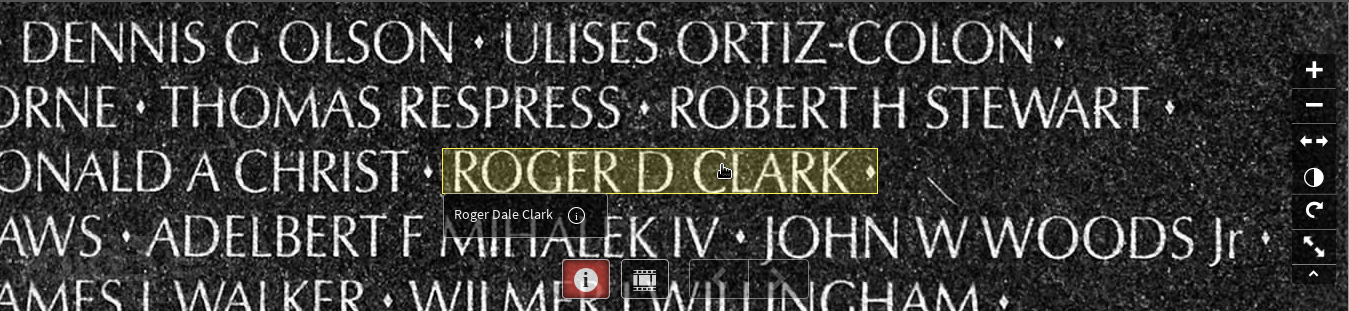
\includegraphics[width=12cm]{fold3.png}}
    \caption{Vietnam Memorial page at fold3.com}
    \label{Vietnam Memorial inspiration}
    \end{figure}
    
    Insipration for my site design was provided by the vietnam memorial application at fold3.com.  
    
        My Website overview:
            My website is fairly typical and includes the following:
                Front-End:  Javascript Library: jQuery \& jQueryUI
                
                Back-End:   Operating system:   Arch Linux
                            Web Framework:      Django
                            Web Server:         Gunicorn
                            Web Proxy:          Nginx
                            Database:           PostgreSQL
                
            When the user is browsing an individual page he / she sees a calligraphy page, inside a re-sizable window.
                Green boxes are overlay-ed on top of all characters in this page that map to the Character Database.
                
                The page is naturally navigable with a zoom in/out bar and drag-able window.
                Every-time the page is dragged or the zoom level is changed, all character boxes are adjusted so they stay precisely the same position and size with respect to the parent page.
                
                As the user mouses over a character, it's box turns blue indicating that character is a candidate for selection.
                
                Once a character is selected a slider, it's box turns red. A slider at the bottom of the screen becomes populated with characters which are attributed to that same author
                
                When any character in the slider is clicked it opens up a new browser window showing the parent page.  (I really think an Ajax thing where we load the new image into a side-by-side window would be much better)
                
                This allows another researcher to (hopefully) easily and (also hopefully) comprehensively compare a large number of similar, but different characters, in order to discern the subtle differences between and among Calligraphic works
                
                An image browser using an adaptive scroll bar was something I could not find, so I had to make it.  My origional work based on JRAC, the Jquery Resize And Crop tool.  My improvements constitute the fixed point zoom feature, where the zoom maintains the center of focus on the center of the viewing window.  I accomplished this by having JQuery adjust the location of the image during resize events.  Also, jquery re-calculates the locaiton of every bounding box during both zoom and drag operations.
                
                There are several significant shortcomings in my method though.
                1)  The whole high resolution image is downloaded during page viewing. This causes a significant time period to elapse during page render.
                2)  The bounding boxes are fairly heavyweight javascript objects, My impleentation works well for dozens, but could not sustain thousands.
                3)  The positions of every bounding box are re-calculated and the box positions are updated during zoom and pan operations regardless of zoom level.  At high zoom levels the processor spends significant time on objects that are not visible.
                
                
                    My results:
        *  I created a website that permits browsing uploaded images of calligraphy texts.
            +Bounding boxes are overlay-ed on top of characters on the 
                *These bounding boxes follow characters during navigation (Zoom and drag)
                *Zooming is continuous, not discrete, this way researchers can see the two characters side-by-side for a more effective comparison
            +To the best of my knowledge, this is the first web application to allow easy and direct navigation between similar characters on scanned high resolution, continuously zoom-able images.
            

